\title{Supplementary material}
\author{}
\date{}

\begin{document}
\maketitle



In order to show how we implemented our framework and how model
components are translated into selection and drift dynamics we applied
our approach to simulated communities to address
the following questions:
% performed
% simulations as described below. Our goal is to address main criticisms
% of our framework being:
(1) Are fixed and random effects of our models actually
capturing selection and drift dynamics? (2) Are random effects only
capturing drift dynamics or uninformed species traits are inflating
random effects?


\subsection*{Goals}\label{material-and-methods}
% PI 17 dez 2020: esta seção já me parece metodologia mesmo, e os goasls eriam o que está acima
We use simulated communities assembled by selection and drift dynamics
in order to show how fixed and random effects capture different
ecological processes. Also, we use traits with strong and weak
correlations to species abundance in order to show how fixed and
random effects capture drift dynamics when traits are
uninformative. We thus simulated three scenarios, with the same data
structure as our abundance data of ferns in three mountain chains in
southern Brazil:


\begin{itemize}
\tightlist
\item
  Deterministic community with traits strongly correlated with species abundance from Poisson sample
\item
  Deterministic community with traits poorly correlated with species abundance from Poisson sample
\item
  Stochastic community with traits strongly correlated with species abundance from Poisson sample
\end{itemize}



\subsection*{Building simulated
communities and samples}\label{building-simulated-communities}

We used the R package MCSIM (available at:
\url{https://github.com/sokole/MCSim}) from Eric Sokol to create
simulations of
metacommunities %to test assumptions about their underlying processes underlying
(Sokol et al.~2015). To replicate a data set analogous to our data all
metacommunities were composed by 30 sites in three regions with 153
species. We fixed the total number of individuals in the metacommunity
as 1,000,000 and migration parameter at 0.5.

Deterministic communities
were modelled based on an environmental gradient that weights the
selection of colonizers of each site from a common poll, based on how
well fitted each species is to the environmental conditions of each
site.  In addition, deterministic communities exhibit a flat dispersal
kernel, to express that dipsersal is not limited.  For deterministic
communities with strong traits, we defined values of traits that were
highly correlated with the environmental response of each species to
the environmental gradient.

In stochastic communities species are also selected based on the
environmental gradient, however the standard deviation from the mean
response to the gradient is high enougj to emcompass the whole
gradient.  In practice, such arametrization ensues a neutral scenario
(Sokol et al.~2015). Also, stochastic communities exhibit a limited
dispersal kernel, to simulate dispersal limitaion among sites and more
strongly among regions.

For each scenario we generated 100 communities and then we simulated
Poisson samples from each community to build data sets used in our
model selection framework. Each sample had on avreage 20,000
individuals (that is, 2\% of the total number of individuals).

\subsection*{Fitting models to simulated
data}\label{fitting-models-to-simulated-data}

We used our framework to fit models to the sample abundances of each
community in the three scenarios. We then calculated the proportion of
simulations that resulted in which each each model was well supported
by the data \(\Delta{AIC} < 2\). We also calculated the adjusted
\(R^{2}\) for the selected models, from code adapted from Johnson
(2014), to calculate: (i) marginal and conditional \(R^{2}\) of each
model, (ii) enhanced agreement repeatibility (Stofel et al
2107). Agrrement repeatability can is the ratio of the intra-class
variance for a given random factor and the total variance estimated by
the models, including fixed-effect variances. These functions are
available in the script \texttt{functions.R} accompanying this text, but
applies only to models within our framework. % PI 17 dez 2020:  ao framework ou aos modelos do nosso estduo de caso? Acho que é o segundo caso, não?
For generic functions
please see packages (rptR and MuMIn).

\subsection*{Results}\label{results}

Based on our simulations, we found that samples from deterministic
communities with traits highly correlated to abundance provide strong
support for the models that express the Trait-mediated Selection
hypothesis (Table S1). As expected, samples from deterministic
communities with traits poorly correlated to abundance support mainly
the models that correspond to the Selection \& Drift
hypothesis. Samples from stochastic communities are also strongly
support the model that express the Drift hypothesis.

By examining the partition of $R^{2}$ values, we can understand how
selection and drift terms in the best-supported statistical models
capture variance in species abundance
(Figure S1). When comparing deterministic communities with traits
correlated to abundance with stochastic communities, it is clear that
in the first case, most of the $R^{2}$ is accounted by the fixed
effects. In contrast, the variance in the abundance of stochastic
communities is mostly due to the component of regional limited
dispersal (1|SP:R). For deterministic communities with traits poorly
correlated to abundance, we still see that the largest share of the $R^{2}$ 
is for selection terms. However, most of the variation is 
explained by the term (1 + G|SP) which represents the variance of
species abundance in respect to the gradient but independent of the
measured traits. In other words, this term can identify if the model
is being built with the wrong traits.

\begin{table}[!ht]

\caption{\label{tab:table-prop}Proportion of models with {$\Delta$} AIC {$<$}  2 at each scenario.}
\centering
\begin{tabular}[t]{p{3cm}p{2cm}p{2.cm}p{2.cm}p{2cm}p{2cm}p{2cm}}
\toprule
\textbf{Scenario} & \textbf{Trait-mediated Selection} \& \textbf{Drift} & \textbf{Selection \& Drift} & \textbf{Trait-mediated Selection} & \textbf{Selection \& Drift} & \textbf{Drift} & \textbf{Idyosyncratic}\\
\hline
Deterministic with right traits & 1.00 & 0.00 & 0 & 0.00 & 0 & 0\\
Deterministic with wrong traits & 0.00 & 0.82 & 0 & 0.18 & 0 & 0\\
Stochastic with right traits & 0.02 & 0.00 & 0 & 0.00 & 1 & 0\\
\bottomrule
\end{tabular}
\end{table}

\begin{figure}
\centering
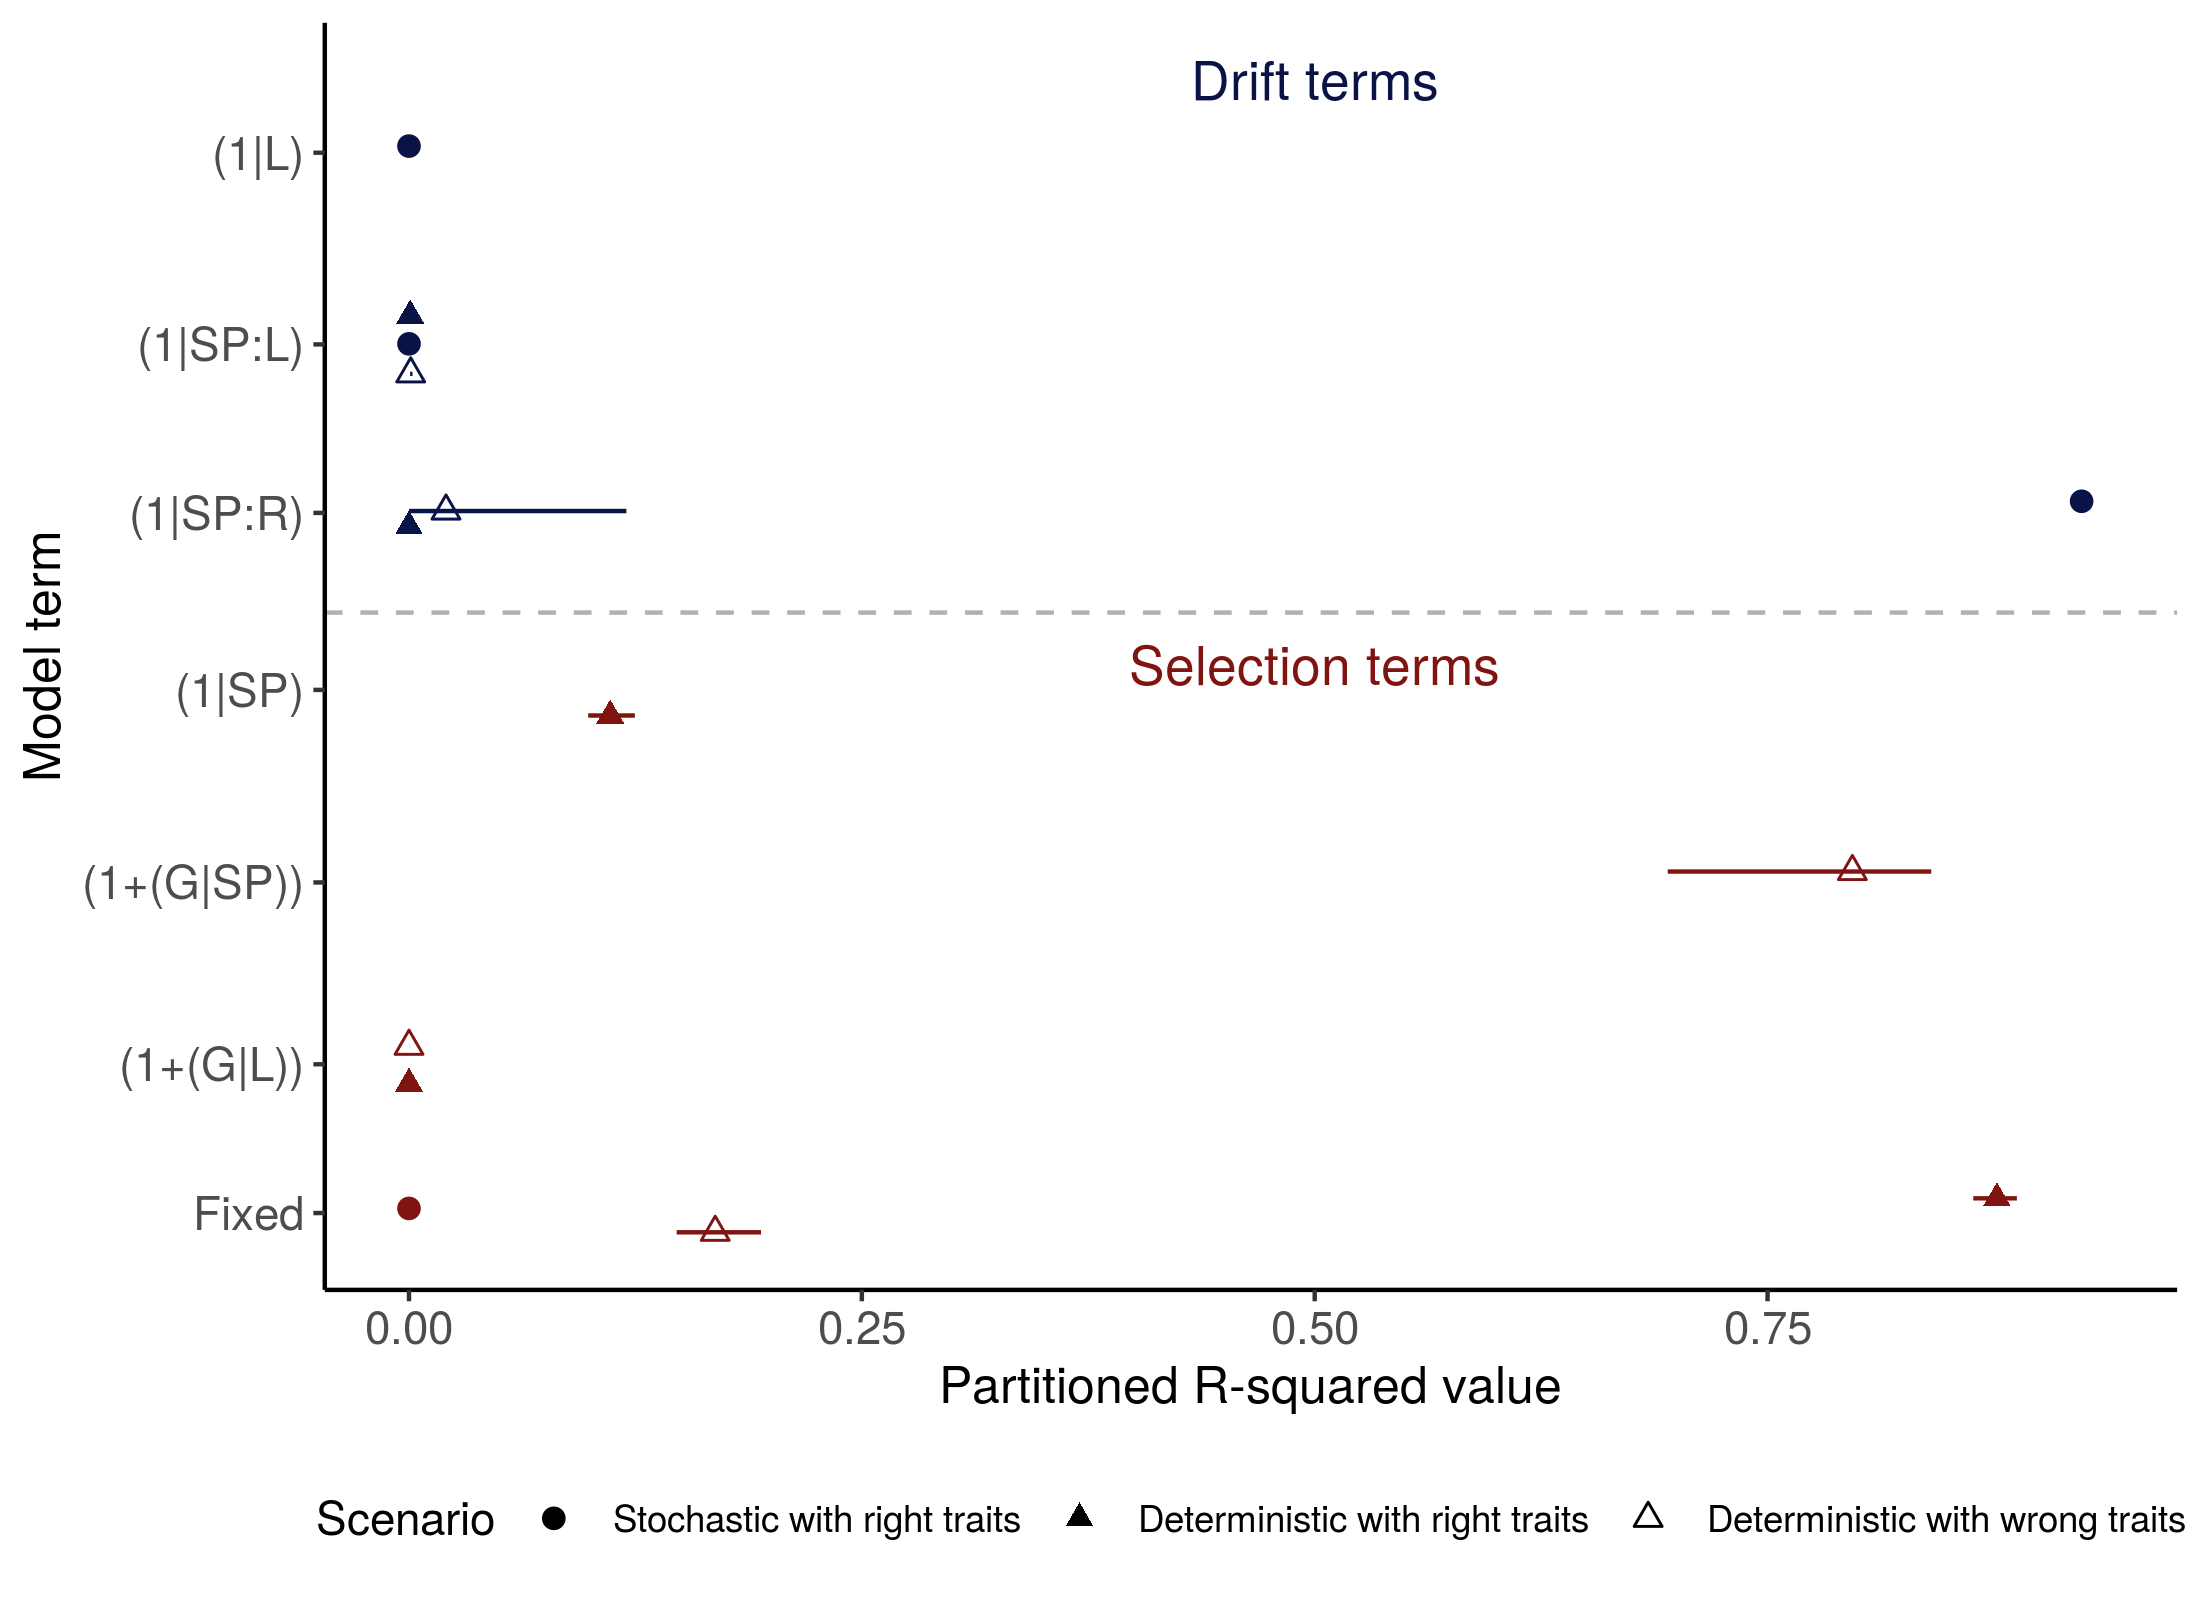
\includegraphics[scale=.9]{fig/S1.png}
\caption{Figure S1.}\label{fig:r2}
\end{figure}

\end{document}
